\section{A Running Example: DrawableDeck}~\label{sec:overview}
This section illustrates the features of our model for
resolving unintentional method conflicts. As mentioned before, such a
case arises when two inherited methods happen to have the same
signature, but with different semantics and functionality. This
situation is troublesome to programmers that use multiple
inheritance. Below we illustrate with a running example called
\lstinline|DrawableDeck|, which models a drawable deck of cards. 
Note that we use Java-like syntax
throughout the paper, and all types are defined with the keyword
``\lstinline|interface|''. The concept is closely related to Java 8
interfaces with default methods~\cite{bono14} and traits. For simplicity, an interface in our model has
the following characteristics:
\begin{itemize}
  \item It allows multiple inheritance.
  \item Every method represents a behaviour and requires a body for its implementation (like Java 8 default methods). There are no abstract methods.
  \item It can be directly instantiated by the \lstinline|new| keyword.
\end{itemize}
Furthermore for simplicity, our examples and formalization does not deal with state at
this stage. %%, but that should not block our discussions below.

\subsection{Problem 1: Unintentional Method Conflicts}
Suppose that two components \lstinline|Deck| and \lstinline|Drawable| 
have been developed in a system.  \lstinline|Deck| represents a deck
of cards, and defines \lstinline|draw| for drawing a card from the
deck.  \lstinline|Drawable| is an interface for graphics that
can be drawn, and also includes a method called \lstinline|draw| for
visual display. For illustration, the implementation of
\lstinline|draw| in \lstinline|Drawable| only creates a blank canvas
on the screen, and later some instances (\lstinline|Circle|,
\lstinline|Square|, or others) that extend \lstinline|Drawable| may
define their own \lstinline|drawObject| methods and invoke
\lstinline|draw|.

\vspace{3pt}\begin{lstlisting}
interface Deck {
  void draw() { // draws a card from the Deck
    Stack<Card> cards = this.getStack();
    if (!cards.isEmpty()) { Card card = cards.pop(); ... }
  }
}

interface Drawable {
  void draw() { // draws something on the screen
    JFrame frame = new JFrame("Canvas");
    frame.setVisible(true);
    ...
  }
}
\end{lstlisting}\vspace{3pt}
Note that both methods have \lstinline|void| return type (we will not formalize
\lstinline|void| in our calculus afterwards; here is only for illustration). In \lstinline|Deck|, \lstinline|draw| tries to get the cards as a stack, pops
out the top card, and so on. While in \lstinline|Drawable|, \lstinline|draw|
creates a blank canvas using \lstinline|JFrame|. Now, a programmer is designing a
card game with GUI. He may want to draw a deck on the screen, so he defines a drawable
deck using multiple inheritance:

\vspace{3pt}\begin{lstlisting}
interface DrawableDeck extends Drawable, Deck {...} 
\end{lstlisting}\vspace{3pt}
The point of using multiple inheritance is surely for composing the features from various 
components, and to achieve code reuse, as supported by many mainstream OO
languages. Nevertheless at this point, languages like Java simply throw a compile
error on \lstinline|DrawableDeck|, since the two \lstinline|draw| methods cause a conflict, though accidentally.

Now one may quickly comes up with a workaround, which is creating a new \lstinline|draw| in \lstinline|DrawableDeck| to
explicitly overrides the old ones. However, the two conflicting methods have totally different functionalities, merging
them into one does not make any sense. This non-solution will hide the old methods, and break independent extensibility. The
feature we expect is called ``triangle inheritance'', that is to say, when the conflicting methods serve for different behaviours,
we can allow them to coexist in the extending interface in a type-safe way.\\

\noindent\textbf{Potential Fixes} There are several workarounds that come to our mind:
\begin{itemize}
  \item \textbf{I. Delegation.} As an alternative to multiple inheritance,
  delegation can be used by introducing two fields with
  \lstinline|Drawable| type and \lstinline|Deck| type,
  respectively. This avoids method conflicts. Nevertheless, it is known
  that using delegation makes it hard to correctly maintain
  self-references \haoyuan{need to cite} in an extensible system [], and also
  introduces a lot of boilerplate code.
  \item \textbf{II. Refactor Drawable and/or Deck to rename the methods.} If
  the code for \lstinline|Drawable| or \lstinline|Deck| are available
  then it may be possible to rename one of the \lstinline|draw|
  methods. However this approach is non-modular, as it requires 
  modifying existing code, and may not be possible if code is unavailable.
  \item \textbf{III. Method exclusion/renaming in traits.} Some trait models
  support method exclusion/renaming. Those features
  provided can eliminate conflicts, although most
  programming languages do not support them. In a traditional OO system,
  they can break the subtyping. Moreover, in
  contrast with exclusion, renaming can indeed preserve both conflicting
  behaviours, however, it is cumbersome in practice, as introducing new
  names can affect other code blocks.
  \item \textbf{IV. Static dispatch.} Some other languages like C++ have
  direct support for the triangle inheritance. While conflicting methods are
  both preserved, the ambiguity of method call is resolved by static dispatch.
  Qualified names are used to specify the branch to give the right implementation.
\end{itemize}

\noindent\textbf{Our solution:} below is our code that shows the triangle
inheritance.
We can define \lstinline|DrawableDeck| by inheriting \lstinline|Drawable| and \lstinline|Deck| together while
type safety is ensured. Again it is slightly different from our prototype as we do not model \lstinline|void| or statements;
the code is just for illustration.
\vspace{3pt}\begin{lstlisting}
interface DrawableDeck extends Drawable, Deck {}

interface Foo {
  void func(Deck obj) { obj.draw(); }
}

// main program
DrawableDeck d = new DrawableDeck();
new DrawableDeck().Drawable::draw();      // calling draw in Drawable
new Foo().func(new DrawableDeck());       // calling draw in Deck
\end{lstlisting}\vspace{3pt}
Note that both cases in the above code are valid in C++ for disambiguation. As shown by \lstinline|func|, C++ looks at
the static type of the receiver for static dispatching. Normally we can define such a method \lstinline|func| for ``implicit''
casts in \name{}. C++ further allows explicit casts.

In the following text we will see that C++ is still unsatisfactory, as it introduces another problem on code reuse, which motivates
our work.

\subsection{Problem 2: Dynamic Dispatch for Code Reuse}\label{subsec:problem2}

\bruno{Emphasizing hierarchical dispatch and triangle inheritance.}\haoyuan{Done}
On the other hand, we also need dynamic dispatch as it is essential and widely used in object-oriented programming.
C++ has the flexibility for choosing either way of dispatch by the \kwvirtual{} keyword.
Unfortunately, this approach is still unsatisfactory regarding code reuse. For instance, 
we redefine \lstinline|Deck| to support
both \lstinline|draw| and another operation called \lstinline|shuffleAndDraw|:
\vspace{3pt}\begin{lstlisting}
interface Deck {
  void draw() {...}
  void shuffleAndDraw() { shuffle(); draw(); }
  ...
}
\end{lstlisting}\vspace{3pt}
\lstinline|shuffleAndDraw| is a typical method that invokes \lstinline|draw| in its definition. In principle, we want
that invocation to use dynamic dispatch, because a programmer may define a subtype of \lstinline|Deck|, and override \lstinline|draw|:
\vspace{3pt}\begin{lstlisting}
interface LoggingDeck extends Deck {
  void draw() { // overriding
    Stack<Card> cards = this.getStack();
    if (!cards.isEmpty()) {
      Card card = cards.pop();
      println("The card is: " + card.toString());
      ...
    } else println("Empty deck.");
  }
}
\end{lstlisting}\vspace{3pt}
In that case, \lstinline|shuffleAndDraw| needs to be adapted to the new \lstinline|draw|. But due to static dispatch,
it still refers to the old \lstinline|draw| in \lstinline|Deck|. Thus programmers have to copy the \lstinline|shuffleAndDraw| code in
\lstinline|LoggingDeck|. It requires a lot of redundant work if we have to duplicate all such methods. Hence in order for code reuse,
we cannot just rely on static dispatch. However, as seen before, dynamic dispatch would take us back to problem 1, for instance, when we
have the UML in Figure~\ref{fig:drawableloggingdeck} and the following code:
\vspace{3pt}\begin{lstlisting}
interface DrawableLoggingDeck extends Drawable, LoggingDeck {...}

// main program
DrawableLoggingDeck d = new DrawableLoggingDeck();
d.shuffleAndDraw(); // ambiguous draw if dynamically dispatched
\end{lstlisting}\vspace{3pt}

\begin{figure*}[t]
  \centering
  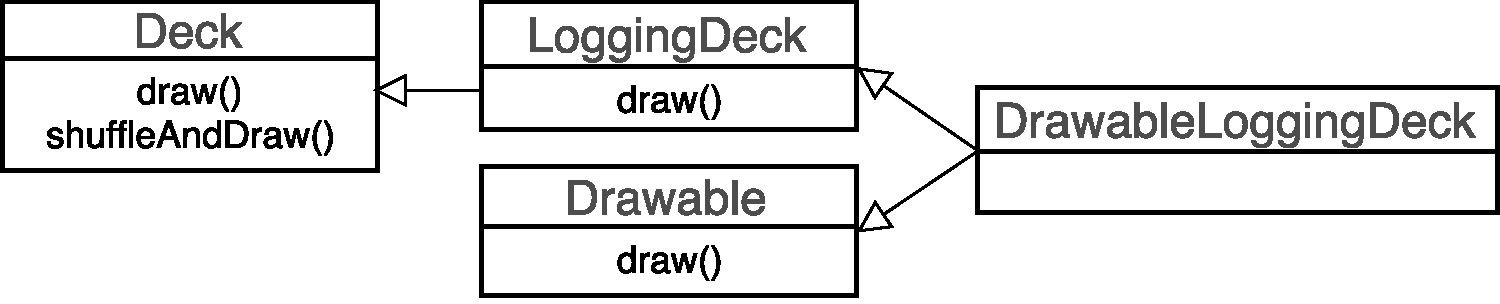
\includegraphics[height=2cm]{pics/DrawableLoggingDeck.pdf}
  \caption{UML graph for \lstinline|DrawableLoggingDeck|.}\label{fig:drawableloggingdeck}
\end{figure*}
If we try to keep the triangle inheritance, but apply dynamic dispatch, calling \lstinline|shuffleAndDraw| would trigger ambiguity. 
In principle we want \lstinline|shuffleAndDraw| to invoke \lstinline|LoggingDeck.draw|, because they belong to the same branch, 
nonetheless, choosing either static dispatch
or dynamic dispatch cannot ensure both the triangle inheritance and code reuse. As far as we know, C++ does not have a solution
to it. Therefore we need to find another algorithm for method resolution.\\

\noindent\textbf{Our solution:} we propose \textit{hierarchical dispatch} for method lookup. A qualified
method invocation in our model, for instance, \lstinline|e.I::m()|, is read as
``finding the most specific method \lstinline|m| along the path
\lstinline|I|''. The meaning of ``along the path \lstinline|I|'' is
that, if the result of \dispatch{} is \lstinline|J.m()| for some \lstinline|J|, then such a \lstinline|J| must be a super type of \lstinline|e|'s dynamic type, and \lstinline|J| has a subtyping relation with \lstinline|I| (either \lstinline|J <: I| or \lstinline|J >: I|). Intuitively, the most specific \lstinline|m()| must be from branch \lstinline|I|, but it can be an updated version after \lstinline|I| because of dynamic dispatch. The formal definition will be introduced later.

On the other hand, \lstinline|e.m()| where \lstinline|e| has static type \lstinline|I|, simply behaves the same as \lstinline|e.I::m()| in our model. Such a dispatch algorithm makes use of both the static type and the dynamic type of the receiver, so it is like a combination of static and dynamic dispatch. Intuitively, the static type specifies one branch to avoid ambiguity, and the dynamic type finds the latest version on that branch. It may still introduce ambiguity when there are multiple paths from the static type to the dynamic type, and those paths cause conflicts. We disallow this kind of conflict to ensure unambiguity. That is to say, we do not allow two methods to override a same base method when they cause conflicts. This is natural, as they are just two versions of the same operation, hence it is no longer an ``unintentional'' conflict, but the diamond problem.

Back to the example, we can write \lstinline|"this.Deck::draw()"| inside the implementation of \lstinline|shuffleAndDraw|, and on \lstinline|d.shuffleAndDraw()| it automatically dispatches to \lstinline|LoggingDeck.draw()|. Furthermore, the following code
also behaves as expected:
\vspace{3pt}\begin{lstlisting}
interface Deck {
  void draw() {...}
  void shuffleAndDraw() { shuffle(); draw(); }
  ...
}
\end{lstlisting}\vspace{3pt}
It is because the compiler is able to know that the receiver ``\lstinline|this|'' exactly has static type \lstinline|Deck|. Hence hierarchical dispatch eliminates ambiguity.

\subsection{Problem 3: Overriding on Individual Branches}\label{subsec:partialoverrides}

We have seen that hierarchical dispatch can dynamically find the latest implementation of a method from one path (or branch). But when
several branches are merged by triangle inheritance, there is usually demand for updating them separately. For example, someone plans to
reuse the other features of \lstinline|DrawableLoggingDeck|, but updates the \lstinline|draw| from \lstinline|Drawable| by setting the canvas
invisible. Unfortunately in traditional models, the merged branches cannot be separately overridden any longer, since overriding
will hide all branches and break coexistence. Modifying existing code is again unsatisfactory as it affects modularity.\\

\noindent\textbf{Our solution:} an additional feature of our model is \textit{hierarchical overriding}. It allows conflicting methods
to be overridden on individual branches, and hence offers independent extensibility. The above example can be easily realized by:
\vspace{3pt}\begin{lstlisting}
interface DrawableLoggingDeck2 extends DrawableLoggingDeck {
  void draw() override Drawable {
    JFrame frame = new JFrame("Canvas");
    frame.setVisible(false);
    ...
  }
}

// main program
DrawableLoggingDeck2 d = new DrawableLoggingDeck2();
d.Drawable::draw()      // calling draw in DrawableLoggingDeck2
\end{lstlisting}\vspace{3pt}
\textbf{Terminology} The \lstinline|draw| methods we saw before this example are called ``original methods'' in this paper, because they are originally defined in its interface.
In contrast, \lstinline|DrawableLoggingDeck2| defines a ``hierarchical overriding'' method. The difference is that traditional overriding overrides all branches by defining another original method, whereas hierarchical overriding only refines one branch.

In our model, triangle inheritance allows several original methods (branches) to coexist, and hierarchical dispatch first finds the most specific original method (branch), then it finds the most specific hierarchical overriding on that branch. A quick counter-example is when there are two hierarchical overriding methods on \lstinline|Drawable| in \lstinline|DrawableLoggingDeck2|, it leads to ambiguity. The compiler is supposed to forbid that during compile time.

Two rules for hierarchical overriding: it can only refine \textbf{original} methods, and cannot jump over original methods with the same signature. For instance, writing \lstinline|"void draw()| \lstinline|override Deck {...}"| is disallowed in \lstinline|DrawableLoggingDeck2|, because existing two branches are \lstinline|Drawable.draw| and \lstinline|LoggingDeck.draw|, while \lstinline|Deck.draw| is already covered. It does not really make sense to refine an old branch.

Similar to many OO languages, the model also allows \textit{super method invocation} in a method body. The invocation \lstinline|super.T::m()| will ignore all the subtypes of \lstinline|T|, and only look at \lstinline|T| together with its super interfaces. It should behave the same as \lstinline|new T().m()| in principle.